\begin{exo}
	Dans une ville, une enquête portant sur les habitudes des ménages en matière d'écologie a donné les résultats suivants :
	\begin{itemize}
		\item $70$\% des ménages pratiquent le tri sélectif ;
		\item Parmi les ménages pratiquant le tri sélectif, $40$\% consomment des produits bio ;
		\item Parmi les ménages ne pratiquant pas le tri sélectif, $10$\% consomment des produits bio.
	\end{itemize}

	On choisit un ménage au hasard et on note les événements :

	\begin{itemize}
		\item $T$ : \og{} le ménage pratique le tri sélectif \fg{} ;
		\item $B$ : \og{} le ménage consomme des produits bio \fg{}.
	\end{itemize}

	\begin{enumerate}
		\item \begin{enumerate}
			      \item Déterminer, sans justification, $P(T)$.
			      \item Déterminer, sans justification, les probabilités conditionnelles :
			            \[
				            P_{T}\pa{B}\ \text{ et }\ P_{\overline{T}}\pa{B}
			            \]

		      \end{enumerate}
		\item Représenter la situation à l'aide d'un arbre pondéré.
	\end{enumerate}

	\begin{center}
		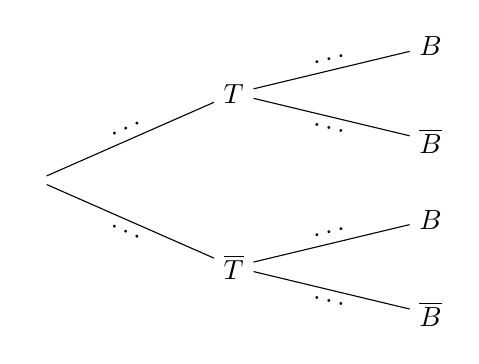
\begin{tikzpicture}[grow=right, sloped, level distance=2.5cm,
				level 1/.style={sibling distance=2.2cm},
				level 2/.style={sibling distance=1.2cm}]

			\node {}
			child {node {$\overline{T}$}
					child {node {$\overline{B}$} edge from parent node[below] {$\ldots$}}
					child {node {$B$} edge from parent node[above] {$\ldots$}}
					edge from parent node[below] {$\ldots$}
				}
			child {node {$T$}
					child {node {$\overline{B}$} edge from parent node[below] {$\ldots$}}
					child {node {$B$} edge from parent node[above] {$\ldots$}}
					edge from parent node[above] {$\ldots$}
				};
		\end{tikzpicture}
	\end{center}

	\ber
	\item
	\begin{enumerate}
		\item Calculer la probabilité de : \og{} le ménage pratique le tri sélectif et consomme des produits bio \fg{}.
		\item Calculer $P\pa{\bar{T}\cap B}$.
	\end{enumerate}
	\end{enumerate}
	L'événement $B$ est formé par la réunion des deux événements incompatibles $T \cap B$ et $\overline{T} \cap B$, on admet que :
	\[ P(B) = P(T \cap B) + P(\overline{T} \cap B) \]
	\ber
	\item Calculer $P\pa{B}$ et vérifier que la probabilité que le ménage consomme des produits bio est égale à $0,31$.
	\item Calculer la probabilité que le ménage pratique le tri sélectif sachant qu'il consomme des produits bio.
	\end{enumerate}
\end{exo}
